\section{The Minimal Supergravity Framework}
We want to include Gravity, or more precisely local Supergravity, in our setting. The relevant physical scale in this context is the Planck scale $M_{\mathrm{Planck}}\sim 10^{19}$ GeV, since it is the scale where the strength of the gravitational interaction is assumed to be of $\mathcal{O}(1)$.
All of the phenomenological problems discussed before are solved at once if one assumes that the MSSM parameters obey a set of boundary conditions at some high-energy scale $M_X$. We will in the following refer to this scale as the \enquote{unification scale}, for reasons that will become clear in the following. These boundary conditions can be implemented quite naturally, when assuming gravity-mediated SUSY breaking in the hidden sector with $m_{\mathrm{soft}}\sim\frac{\langle F\rangle}{M_{\mathrm{Planck}}}$ as discussed at the end of the previous section. The idea is then to access the low-energy MSSM phenomenology via standard renormalization group techniques using these boundary conditions as input parameters. This idea is visualized at the beginning of this page in Figure \ref{fig:msugra}. 
\begin{figure}[t]
\centering
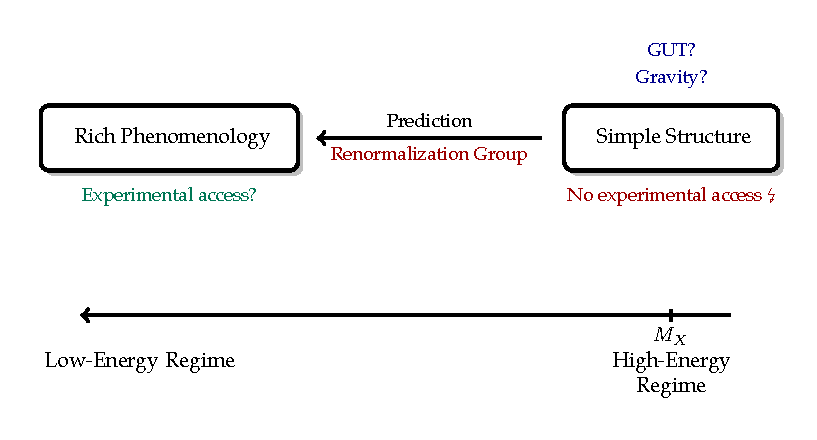
\includegraphics[scale = 1]{figures/mSUGRA_idea}
\caption{An overview of the idea of the mSUGRA framework. Assuming a simple high-energy structure of the theory, we can derive low-energy predictions using standard renormalization group techniques.}
\label{fig:msugra}
\end{figure}\\
\noindent The implementation of the boundary conditions is realized by assuming a \enquote{minimal} normalization of the kinetic terms in the SUGRA Lagrangian:
\begin{equation}
	\mathcal{L}_{\mathrm{SUGRA}} \supset-\frac{1}{M_{\mathrm{Planck}}} F\left(\frac{1}{2}  \alpha\lambda \lambda+\frac{1}{6}  \beta  \phi \phi \phi+\frac{1}{2} \gamma \phi \phi\right)+\mathrm{h.c.}-\frac{1}{M_{\mathrm{Planck}}^{2}} F F^{*} \delta \phi \phi^*.
\end{equation}
Note that we suppressed all the indices for simplicity. A careful comparison with the the initial terms in $\mathcal{L}_{\mathrm{soft}}$ then allows us to find relatively simple relations for the input parameters, i.\,e.
\begin{equation}
	\begin{aligned}
		m_{1/2} &= \alpha\frac{\langle F\rangle}{M_{\mathrm{Planck}}}, \qquad m_{0}^2 = \delta\frac{\abs{\langle F\rangle}^2}{M_{\mathrm{Planck}}^2}\\
		A_0 &= \beta\frac{\langle F\rangle}{M_{\mathrm{Planck}}}, \qquad B_{0} = A_0 - m_0 = \gamma\frac{\langle F\rangle}{M_{\mathrm{Planck}}}.
	\end{aligned}
\end{equation}
This relatively simple structure allows to simplify the structure of the relevant couplings at the initial scale as follows:


\begin{itemize}
		\item The scalar squared-masses are flavor-diagonal and universal: 
	\end{itemize}
	\begin{equation}
	\begin{aligned}
				m^2_{\tilde{q}}(M_X) &= 	m^2_{\tilde{u}}(M_X) = m^2_{\tilde{d}}(M_X) = m_0^2 \mathbb{1} \\[0.5em]
				m^2_{\tilde{\ell}}(M_X) &= 	m^2_{\tilde{e}}(M_X) = m_0^2 \mathbb{1} \\[0.5em]
				m^2_{1}(M_X) &= 	m^2_{2}(M_X) = m_0^2 .
	\end{aligned}
	\end{equation}
		\begin{itemize}
		\item The same is true for the $A$-parameters:
	\end{itemize}
	\begin{equation}
	\begin{aligned}
				A^{U} (M_X) = A^{D} (M_X) = A^{E} (M_X) = A_0^2 \mathbb{1}.
	\end{aligned}
	\end{equation}
	\begin{itemize}
		\item Additionally we assume unification of the (tree level) gaugino masses:
		\end{itemize}
	 \begin{align}
				M_1 (M_X) = M_2 (M_X) = M_3 (M_X) = m_{1/2}. 
	\end{align}
These relations provide our starting point for the subsequent renormalization group evolution towards the low-energy regime. Just as a reminder, we define the beta function as $\beta(g) = \frac{\partial g}{\partial \operatorname{ln} M}$, the rate of change of the renormalized coupling at the scale $M$, where the bare coupling is fixed \cite{PeskinSchroeder1995}. As an example, the RG evolution of the gaugino mass parameters yields the following, well known relation:
\begin{equation}
	M_{i}=\frac{\alpha_{i}\left(M_{Z}\right)}{\alpha_{\mathrm{GUT}}} m_{1 / 2} \longrightarrow M_{3}\left(M_{Z}\right)=\frac{\alpha_{3}\left(M_{Z}\right)}{\alpha_{2}\left(M_{Z}\right)} M_{2}\left(M_{Z}\right)=\frac{\alpha_{3}\left(M_{Z}\right)}{\alpha_{1}\left(M_{Z}\right)} M_{1}\left(M_{Z}\right).
\end{equation}
	This tells us that
	\begin{equation}
		M_{1}=\frac{5}{3} \tan ^{2} \theta_{W} M_{2} \sim \frac{1}{2} M_{2},
\end{equation}
where the factor $\frac{5}{3}$ comes from the unification scheme in our SU(5) model, i.\,e.
\begin{equation}
	g\cdot Y_{\mathrm{GUT}} = g_Y\cdot Y \implies \frac{g}{g_Y} = \sqrt{\frac{5}{3}} 
\end{equation}
and $\theta_{\mathrm{W}}$ is the Weinberg angle measured to be $\sin^2 \theta_{\mathrm{W}} \approx 0.23$.\\
To visualize the general idea on how to get a rich phenomenological low-energy MSSM spectrum from only a few input parameters according to the scheme described beforehand, have a look at Figure \ref{fig:rge} at the beginning of the next page.\newpage
\begin{figure}[t]
\centering
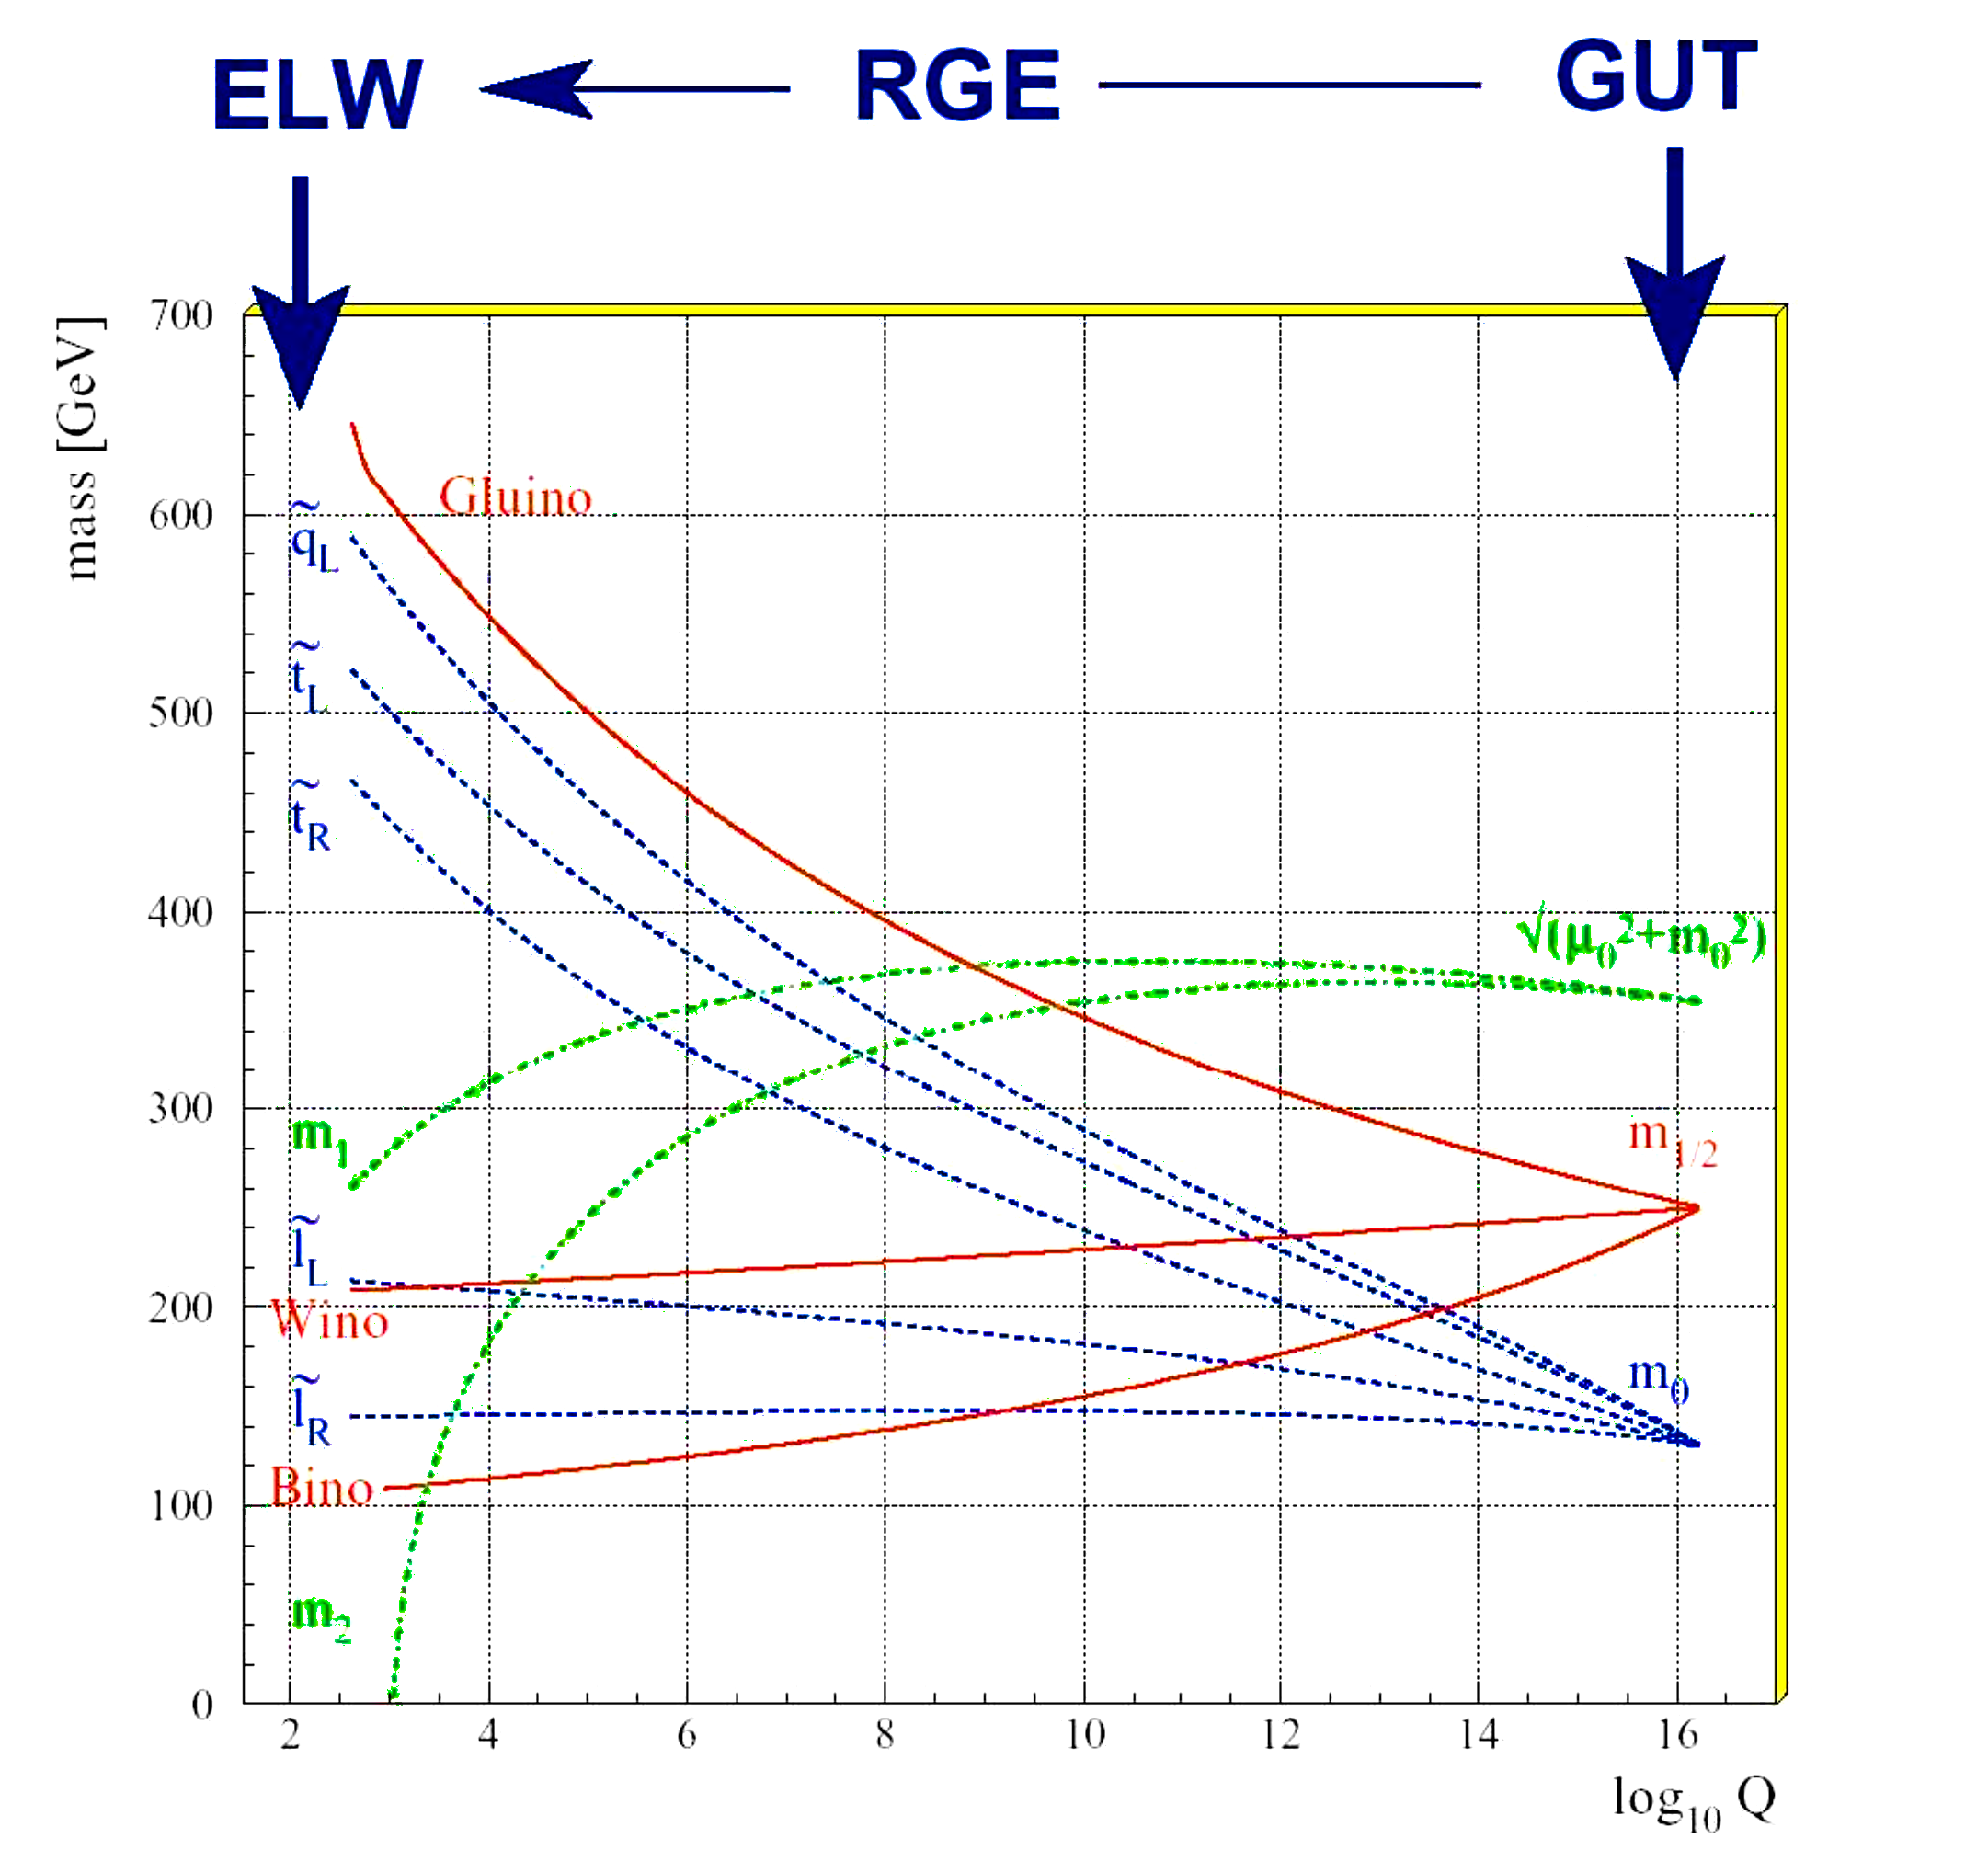
\includegraphics[scale = 0.8]{figures/mSUGRA_RGE}
\caption[Running of the relevant parameters in the mSUGRA approach.]{Running of the relevant parameters in the mSUGRA approach\footnotemark.}
\label{fig:rge}
\end{figure}
\footnotetext{Figure taken from: \tiny\url{https://www.physi.uni-heidelberg.de/~uwer/lectures/ParticlePhysics/Vorlesung/Lect-10b.pdf} (10.02.21)}

\noindent A final parameter count yields that the mSUGRA model only needs four additional continuous and one additional discrete parameter to be entirely characterized:
\begin{itemize}
	\item $\tan\beta$, the ratio of the VEVs in the two-Higgs doublet model.
	\item $m_{1/2}$, the universal gaugino mass.
	\item $m_{0}$, the universal scalar (sfermion/Higgs) mass.
	\item $A_{0}$, the universal trilinear coupling.
	\item $\operatorname{sign}(\mu)$, the sign of the Higgs-higgsino mass parameter.
\end{itemize}
The relations for $\tan\beta$ and $\abs{\mu}$ come from the two minimum conditions for the Higgs potential\footnote{At this point we have to assume that electroweak symmetry breaking occurs which directly lead us to these conditions.}:
\begin{align}
	m_Z^2 &= \frac{m_{H_d}^2 + \mu^2 - (m_{H_u}^2 + \mu^2)\tan^2\beta}{\tan^2\beta -1} \\
	\sin^2 2\beta &= \frac{B_0\mu}{m_{H_u}^2 + m_{H_d}^2 + \mu^2}
\end{align}
Additional constraints such as the unification of the top, bottom and tau Yukawa couplings at the GUT scale can further restrict the possible values of $\tan\beta$ and $A_0$.\\ In total we can conclude that the mSUGRA framework provides a promising candidate for a phenomenologically accessible SUSY model that may be tested in current or future experiment. \\ Since the concept of unification may play a central role in the discussion of SUSY phenomenology, but is often not part of the standard curriculum of Particle Physics or Quantum Field Theory lectures we want to discuss it in more detail in the next section.